\subsection{Single Cycle Architecture}
\label{subsection:single_cycle}
The simplest architecture that can be implemented to execute the ISA previously described is the single cycle architecture in which every clock cycle can be carried out one instruction.
\begin{figure}[h]
  \center
  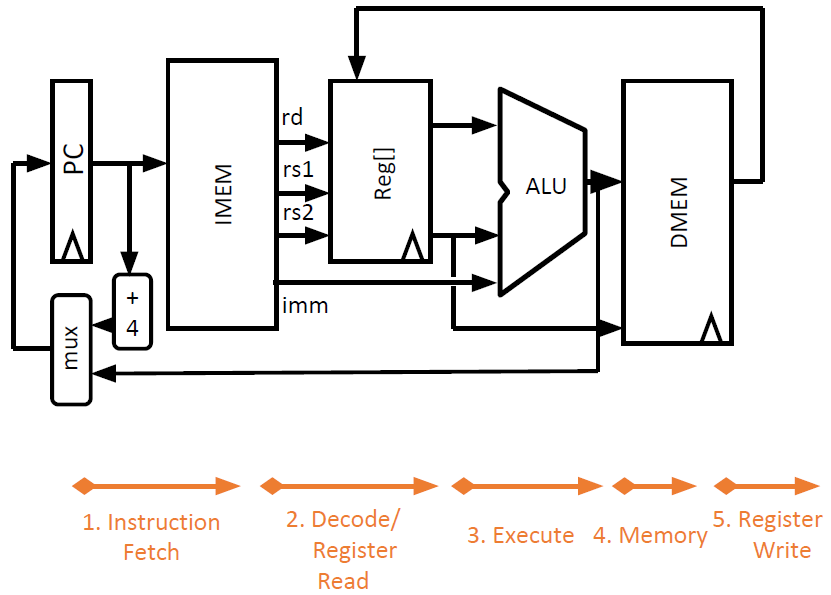
\includegraphics[width=0.7\textwidth]{sec1/images/single_cycle.png}
  \caption{Single Cycle Architecture}
  \label{fig:single_cycle}
\end{figure}
As shown in \autoref{fig:single_cycle}, it is noticeable that this type of processor has separate instruction memory and data memory, which is typical of a Harvard architecture. In order to access the right instruction, there is a dedicated PC register with a mux at its input capable of choosing the right address in case of linear or jump execution. The internal registers are organised in a register file with 32 synchronous write and asynchronous read addresses capable of reading two operands at a time. Finally, there is an ALU with two inputs capable of performing the required arithmetic operations.
In the RISC-V architecture, the execution of an instruction can be divided into five stages:

\begin{description}
    \item \textbf{Fetch:} The instruction is taken from instruction memory.
    \item \textbf{Decode:} The instruction is classified into the various types described in \autoref{subsection:ISA} by the control unit, which generates the control signals necessary for execution. Data from the register file is also read at this stage.
    \item \textbf{Execute:} Arithmetic operations are performed on the operands.
    \item \textbf{Memory:} If necessary, the data memory is accessed to read or write results.
    \item \textbf{Register write:} The result obtained in the execute stage is stored in the register file.
\end{description}
